\documentclass[11pt]{article}
\usepackage[T1]{fontenc}
\usepackage{lmodern,amsmath,amssymb,amsthm,mathtools,booktabs,array,graphicx}
\usepackage[margin=1in]{geometry}
\usepackage{microtype,xcolor,enumitem}
\usepackage[pdfencoding=auto,psdextra,hidelinks]{hyperref}
\hypersetup{pdftitle={A cubic logarithmic law for merging prime-counting scales},pdfauthor={Research note}}
\definecolor{ink}{HTML}{164F61}
\usepackage{fancyhdr}
\pagestyle{fancy}\fancyhf{}
\fancyhead[L]{\small Merging prime-counting scales}
\fancyhead[R]{\small Research note, 26 November 2026}
\fancyfoot[C]{\thepage}
\setlength{\headheight}{14pt}
\setlength{\emergencystretch}{2em}
\allowdisplaybreaks[2]
\newtheorem{theorem}{Theorem}[section]
\newtheorem{lemma}[theorem]{Lemma}
\newtheorem{proposition}[theorem]{Proposition}
\newtheorem{corollary}[theorem]{Corollary}
\theoremstyle{definition}\newtheorem{definition}[theorem]{Definition}
\theoremstyle{remark}\newtheorem{remark}[theorem]{Remark}
\newcommand{\R}{\mathbb R}
\newcommand{\C}{\mathbb C}
\newcommand{\dd}{\,\mathrm d}
\newcommand{\eps}{\varepsilon}
\newcommand{\one}{\mathbf1}
\newcommand{\tr}{\mathsf T}
\newcommand{\dist}{\mathrm{dist}}
\newcommand{\sinc}{\operatorname{sinc}}
\newcommand{\tauE}{\tau_\eps}
\newcommand{\cE}{C_\eps}
\newcommand{\bB}{\mathcal B}
\DeclareMathOperator{\diag}{diag}
\DeclareMathOperator{\spanop}{span}
\title{\textcolor{ink}{A cubic logarithmic law for\\merging prime-counting scales}\\[5pt]
\large Sharp covariance rates, explicit multiplicity bounds,\\and saturation of finite linear prediction}
\author{Research note}
\date{26 November 2026}

\begin{document}
\maketitle
\begin{abstract}
The native smoothing in the final analytic reduction of the Lean proof of
Dirichlet GRH leads to a prime-error signal whose spectral coefficient at a
zeta-zero ordinate $\gamma$ is its multiplicity divided by $1/4+\gamma^2$.
For $r$ observations at logarithmic shifts $\eps u_1,\ldots,\eps u_r$, with
fixed distinct real offsets, we prove that their limiting covariance has
one eigenvalue of order $1$, one of order $\eps^2$, and all remaining
eigenvalues of order $\eps^3\log(1/\eps)$. We give explicit leading-constant
brackets: the small eigenvalues lie asymptotically between those of a
positive cubic-spline form and $4/3$ times those values. No simplicity or
independence of the zeros, and no pair-correlation conjecture, is assumed.
The essential arithmetic step localizes Montgomery's proved
squared-multiplicity estimate by subtracting two pair sums with the same
nonnegative kernel. Every fixed raw finite difference of order at least
two has this same cubic logarithmic variance rate. Optimal prediction
from any fixed number of at least two nearby observations cannot improve
that order, even with coefficients depending on $\eps$. These results
answer the scalar case of an explicit scale-merging question in the
ProveIt multiscale-covariance packet. The new contribution is this
arithmetic logarithmic law and its treatment of multiplicities; the
underlying spline geometry and general kernel-matrix asymptotics have
classical antecedents. Complete ordinary mathematical proofs and
reproducible finite checks are provided; this note is not a new Lean
formalization.
\end{abstract}
\begingroup
\small
\setcounter{tocdepth}{1}
\makeatletter
\renewcommand{\l@section}{\@dottedtocline{1}{0em}{1.7em}}
\makeatother
\tableofcontents
\endgroup
\newpage

\section{Source analysis and the contribution}
\subsection{The inspected RH and GRH interface}
We inspected \texttt{lsernau/grh-lean} at commit
\texttt{72fead102f663d5c7a407964a13dc0cf9d977207} \cite{grh}.
Its \path{grh/src/Statements.lean} uses Mathlib definitions to fix four
explicit zero statements. Its \path{grh/src/Main.lean} exports these and
Mathlib's \texttt{RiemannHypothesis}. The scope is the Riemann zeta function
and Dirichlet $L$-functions, including induced characters; an assertion
about arbitrary Artin or automorphic $L$-functions is not part of this
interface. The project pins Lean~4.35.0 and Mathlib commit
\texttt{56a005855ea17e0b0958f73ec801ae140b0a1679}.

The repository reports the standard three axioms
\texttt{propext}, \texttt{Classical.choice}, and \texttt{Quot.sound}.
Sutherland's independent verification report records builds, statement
comparisons and external-kernel checks \cite{sutherland}. We therefore
use the supplied RH theorem as an established input. We did not rebuild
the entire upstream development in this session, and do not claim a
complete human audit of its approximately 300,000-line readable edition.

The top-level proof compares upper and lower bounds for a normalized Gram
determinant, with lattice-index corrections. Short forms, sufficiently
many forms, and a lower bound for integral forms cancel a common main
term, giving a one-sided smoothed prime estimate. A Landau-type analytic
criterion then excludes zeros to the right of the critical line. Our
result uses the same smoothing and the resulting critical-line spectrum;
it does not claim to extend the theta-lift or arithmetic-geometric part
of that proof. The requested Wikipedia page supplied the overview of
the current status and the prime/zero correspondence \cite{wiki}; the
mathematical inputs below are cited to primary sources.

\subsection{What was already in ProveIt}
At ProveIt commit \texttt{2ccd1e24d0f3fa8a5268c864f66a6b1b4e2d0d59},
the requested directory catalogs 61 placed research packets \cite{catalogue}.
Its nested \path{docs/incoming/} contains a further 29 archives.
Their delivery READMEs and LaTeX texts were screened, with closer reading
of the covariance, spectral-rigidity and inverse-zero results. This was a
novelty screen, not a certification of every earlier proof.

The closest predecessor is \emph{Strict multiscale covariance of smoothed
prime errors}, in \path{grh_multiscale_covariance.zip} \cite{prior}.
It proves positive definiteness for arbitrary fixed distinct scales,
including finite deletion of zero frequencies, and asks:
\begin{quote}
What is the sharp decay as two scales merge?
\end{quote}
The present paper resolves the scalar, modulus-one version for any fixed
number of scales. We rederive the needed scalar explicit formula, so
the new proof does not depend on accepting the predecessor's stronger
multicharacter theorem.

The broad eigenvalue hierarchy for finitely smooth kernels and the role
of compressed distance matrices are prior work of Barthelm\'e and
Usevich and others \cite{BU}. Their quoted finite-smoothness results use
power expansions; the present logarithmic scale and the arithmetic
multiplicity analysis require an additional argument. We claim as a
candidate new result the specific prime-error theorem proved here,
including the localized multiplicity comparison and prediction bounds.
A targeted search and the repository screen found no identical
statement. This is not an exhaustive proof of bibliographic priority.

\section{Definitions and main result}
Let $\Lambda(n)$ be the von Mangoldt function and $\gamma_E$ Euler's
constant. Define, for $x\ge1$ and $t\ge0$,
\begin{align}
 S(x)&=\sum_{n\le x}\Lambda(n)\left(\frac1n-\frac1x\right),\label{eq:S}\\
 E(t)&=e^{t/2}\bigl(S(e^t)-t+\gamma_E+1\bigr).\label{eq:E}
\end{align}
Thus $E$ is a normalized, smoothed prime-power counting error. Its
observations at $t+\eps u_j$ correspond to arguments $x e^{\eps u_j}$.

Throughout, $\gamma>0$ ranges over \emph{distinct} positive ordinates of
the nontrivial zeta zeros, and $m_\gamma$ is the multiplicity of
$1/2+i\gamma$. Write
\begin{align}
 N(T)&=\sum_{0<\gamma\le T}m_\gamma,&
 M_2(T)&=\sum_{0<\gamma\le T}m_\gamma^2.\label{eq:counts}
\end{align}
The following kernel and its first two spectral moments are finite:
\begin{align}
 C(h)&=2\sum_{\gamma>0}
       \frac{m_\gamma^2\cos(\gamma h)}{(1/4+\gamma^2)^2},\label{eq:C}\\
 C_0&=C(0)>0,&
 D&=2\sum_{\gamma>0}\frac{m_\gamma^2\gamma^2}{(1/4+\gamma^2)^2}>0.
 \label{eq:CD}
\end{align}
Their convergence follows from the counting bounds proved or recalled
in Section~\ref{sec:local}. Squaring the multiplicity in \eqref{eq:C}
is essential: coincident frequencies combine before the covariance is
formed.

Fix distinct real $u_1,\ldots,u_r$, $r\ge3$, and put
\begin{align}
 G_\eps&=\bigl(C(\eps(u_i-u_j))\bigr)_{1\le i,j\le r},&
 \tauE&=\eps^3\log(1/\eps),\quad 0<\eps<1,\label{eq:G}\\
 v&=u-\bar u\one,& \bar u&=\frac1r\sum_i u_i,\\
 W&=\{c\in\R^r:c\cdot\one=c\cdot u=0\}.\label{eq:W}
\end{align}
For $c\in W$, define the compactly supported piecewise linear function
and its energy
\begin{align}
 H_c(t)&=\sum_i c_i(t-u_i)_+,&
 \bB(c)&=\int_\R H_c(t)^2\dd t
       =\frac1{12}\sum_{i,j}c_i c_j|u_i-u_j|^3.\label{eq:B}
\end{align}
The identity and strict positivity of this quadratic form are proved in
Lemma~\ref{lem:spline}. Let $B$ be its matrix on $W$ in an orthonormal
basis, and let $b_1\ge\cdots\ge b_{r-2}>0$ be its eigenvalues.
The numbers $b_j$ depend only on the observation offsets and are
computable from a finite matrix.

\begin{theorem}[Arithmetic coalescence law]\label{thm:main}
Using RH, the long-time covariance of
$(E(t+\eps u_1),\ldots,E(t+\eps u_r))$ is $G_\eps$.
The long-time limit is taken first, with $\eps$ fixed. As $\eps\downarrow0$:
\begin{enumerate}[label=(\roman*),leftmargin=*]
\item Uniformly for $c$ in the unit sphere of $W$,
\begin{equation}\label{eq:bracket}
 \bB(c)-o(1)\ \le\ \frac{c^\tr G_\eps c}{\tauE}
 \ \le\ \frac43\bB(c)+o(1).
\end{equation}
Equivalently, the compression to $W$ lies between
$B-o(1)I_W$ and $(4/3)B+o(1)I_W$ after division by $\tauE$.
\item For the eigenvalues in decreasing order,
\begin{align}
 \lambda_1(G_\eps)&\sim rC_0,\label{eq:large1}\\
 \lambda_2(G_\eps)&\sim D\|v\|^2\eps^2,\label{eq:large2}\\
 b_j&\le\liminf_{\eps\downarrow0}\frac{\lambda_{j+2}(G_\eps)}{\tauE}
 \le\limsup_{\eps\downarrow0}\frac{\lambda_{j+2}(G_\eps)}{\tauE}
 \le\frac43 b_j \quad(1\le j\le r-2).\label{eq:small}
\end{align}
In particular all the last $r-2$ eigenvalues have order $\tauE$.
\item The determinant and Euclidean condition number satisfy
\begin{align}
 \det G_\eps&=\Theta_u\!\left(
      \eps^{3r-4}\log(1/\eps)^{r-2}\right),\label{eq:det}\\
 \operatorname{cond}_2(G_\eps)&=
      \Theta_u\!\left(\eps^{-3}/\log(1/\eps)\right).
\end{align}
All conclusions persist after deleting any fixed finite set of positive
zero ordinates, together with their negative partners. The constants
$C_0,D$ change, while $B$ and the factor $4/3$ do not.
\end{enumerate}
No hypothesis of simple zeros, independent ordinates, or the
pair-correlation conjecture is used. The rate is sharp; $4/3$ is a
convenient explicit upper comparison, not an assertion of the optimal
numerical factor.
\end{theorem}

The notation $\Theta_u$ means two positive bounds with constants allowed
to depend on the fixed offsets. With two distinct offsets only,
\eqref{eq:large1}--\eqref{eq:large2} still hold; there is no cubic group.
The case $r=1$ is simply the positive variance $C_0$.

\section{From the prime sum to its covariance}\label{sec:signal}
We record the scalar derivation to make the signs and normalization
independent of the earlier packet. Let
$F(s)=-\zeta'(s)/\zeta(s)$. For $c>1$, Mellin inversion gives
\begin{equation}\label{eq:mellin}
 S(x)=\frac1{2\pi i}\int_{c-i\infty}^{c+i\infty}
      \frac{F(s)x^{s-1}}{s(s-1)}\dd s.
\end{equation}
The inverse kernel is $(x/n-1)_+$ multiplied by $x^{-1}$.
It is zero at $n=x$, so no endpoint convention is needed.

Move the contour to $\Re s=1/4$. Under RH the logarithmic derivative on
this line is $O(\log(2+|\Im s|))$, using its usual local partial fractions
and the local zero-count estimate. The resulting vertical integral is
absolutely convergent and $O(x^{-3/4})$. Horizontal edges can be taken
at heights a distance $\gg1/\log T$ from the zeros; the corresponding
bound is $O(\log^2 T)$ and their integrals vanish. These are the standard
contour estimates underlying the explicit formula; see \cite{kouk}.

At $s=1$, the expansion
$F(s)=1/(s-1)-\gamma_E+O(s-1)$ gives the residue
$\log x-\gamma_E-1$. At $\rho=1/2+i\gamma$, the residue is
\[
 -\frac{m_\gamma x^{\rho-1}}{\rho(\rho-1)}
 =\frac{m_\gamma x^{-1/2+i\gamma}}{1/4+\gamma^2}.
\]
There is no central zeta zero: the positive alternating eta series at
$1/2$ and $\zeta(s)=\eta(s)/(1-2^{1-s})$ show
$\zeta(1/2)\ne0$. Consequently
\begin{equation}\label{eq:series}
 E(t)=P(t)+O(e^{-t/4}),\qquad
 P(t)=2\sum_{\gamma>0}\frac{m_\gamma\cos(\gamma t)}{1/4+\gamma^2}.
\end{equation}
The series is absolutely and uniformly convergent by
$N(T)=O(T\log T)$.

The time mean of $P$ is zero. Multiplying two absolutely convergent
series and taking their time mean leaves only matching opposite
frequencies, proving
\begin{equation}\label{eq:covariance}
 \lim_{T\to\infty}\frac1T\int_{t_0}^{t_0+T}
 E(t+h_i)E(t+h_j)\dd t=C(h_i-h_j).
\end{equation}
Here $t_0$ is any fixed value making the arguments nonnegative.
The exponentially decaying error in \eqref{eq:series} contributes zero
to the limit. Centering by the time means has the same limit. This is a
deterministic long-log-time covariance; no random phases or Gaussian
law are being assumed.

\section{Localized control of squared multiplicities}\label{sec:local}
Riemann--von Mangoldt gives
\begin{equation}\label{eq:RVM}
 N(T)=\frac{T}{2\pi}\log\frac{T}{2\pi}-\frac{T}{2\pi}+O(\log T).
\end{equation}
The traditional consequence of Montgomery's proved theorem under RH is
$M_2(T)\le(4/3+o(1))N(T)$ \cite{montgomery,CGG}. A cumulative upper bound
alone does not compare arbitrary nonmonotone spectral test functions.
The local version needed here follows by keeping the pair kernel fixed
while the height cutoff changes.

\begin{lemma}[Local squared-multiplicity comparison]\label{lem:local}
For every fixed $0<a<b$,
\begin{equation}\label{eq:localM}
 b-a\le\liminf_{T\to\infty}
 \frac{M_2(bT)-M_2(aT)}{T\log T/(2\pi)}
 \le\limsup_{T\to\infty}
 \frac{M_2(bT)-M_2(aT)}{T\log T/(2\pi)}
 \le\frac43(b-a).
\end{equation}
In particular $M_2(T)=O(T\log(2+T))$.
\end{lemma}
\begin{proof}
Put $w(y)=4/(4+y^2)$ and $\sinc y=\sin y/y$, with $\sinc0=1$.
All double sums in this proof repeat zeros according to multiplicity.
For $0<\alpha<1$, Montgomery's equation (6) gives
\begin{align}
 S(X,\alpha)&=\sum_{0<\gamma,\gamma'\le X}
   \sinc^2\!\left(\frac\alpha2(\gamma-\gamma')\log X\right)
   w(\gamma-\gamma'),\notag\\
 S(X,\alpha)&=\left(\frac1\alpha+\frac\alpha3+o(1)\right)
                 \frac{X\log X}{2\pi}.\label{eq:mont}
\end{align}
The error is uniform when $\alpha$ varies in a compact subinterval of
$(0,1)$. For completeness, this follows directly from the uniform form
of his theorem: if $F_X(\beta)$ is the normalized pair transform, then
\[
 \frac{S(X,\alpha)}{X\log X/(2\pi)}
 =\frac1{\alpha^2}\int_{-\alpha}^{\alpha}
       (\alpha-|\beta|)F_X(\beta)\dd\beta,
\]
and uniformly on $|\beta|\le1-\delta$,
$F_X(\beta)=(1+o(1))X^{-2|\beta|}\log X+|\beta|+o(1)$.
The spike integrates to
\[
 \frac1\alpha-\frac{1-X^{-2\alpha}}{2\alpha^2\log X},
\]
and the $|\beta|$ term integrates to $\alpha/3$.

Fix $0<\alpha<1$ and define a \emph{single} kernel
\[
 k_T(y)=\sinc^2\!\left(\frac\alpha2 y\log T\right)w(y)\ge0,
 \qquad k_T(0)=1.
\]
Let $S_T(X)=\sum_{0<\gamma,\gamma'\le X}k_T(\gamma-\gamma')$.
For $X=cT$ with $c>0$ fixed, apply \eqref{eq:mont} with
$\alpha_X=\alpha\log T/\log(cT)\to\alpha$. Uniformity gives
\begin{equation}\label{eq:commonkernel}
 S_T(cT)=\left(\frac1\alpha+\frac\alpha3\right)
       \frac{cT\log T}{2\pi}+o(T\log T).
\end{equation}
When $X$ increases from $aT$ to $bT$, the new diagonal pairs at an
ordinate $\gamma$ contribute exactly $m_\gamma^2$; all added off-diagonal
terms are nonnegative. Hence
\[
 M_2(bT)-M_2(aT)\le S_T(bT)-S_T(aT).
\]
Subtract the two \emph{asymptotic equalities} \eqref{eq:commonkernel},
divide by $T\log T/(2\pi)$, take the limsup, and then let
$\alpha\uparrow1$. This proves the upper bound in \eqref{eq:localM}.
The lower bound follows from $m_\gamma^2\ge m_\gamma$ and
\eqref{eq:RVM}. The global estimate follows in the same way by keeping
all diagonal terms in $S(T,\alpha)$, for any one fixed $\alpha\in(0,1)$.
\end{proof}

\begin{remark}
It would be invalid to subtract two upper bounds for $M_2$. The proof
instead subtracts full asymptotics of pair sums whose kernels are
identical. This supplies local control of the spectral measure.
The choice $\alpha\uparrow1$ occurs after the height limit, within the
proved range of Montgomery's theorem. The conjectural range of the pair
correlation is never used.
\end{remark}

\section{The cubic form and the scaled covariance}\label{sec:cubic}
\begin{lemma}[Spline and Fourier identities]\label{lem:spline}
For $c\in W$, $H_c$ has compact support and
\begin{equation}\label{eq:splineid}
 \int_\R H_c(t)^2\dd t
 =\frac1{12}\sum_{i,j}c_ic_j|u_i-u_j|^3
 =\frac1\pi\int_0^\infty
       \frac{|\sum_i c_i e^{iu_i x}|^2}{x^4}\dd x.
\end{equation}
All three quantities are strictly positive for $c\ne0$.
\end{lemma}
\begin{proof}
For $t$ below the smallest node, $H_c(t)=0$. Above the largest node it
is $t\sum c_i-\sum c_i u_i=0$. Put
$J_c(t)=\sum_i c_i|t-u_i|^3$. The two moment cancellations give
$J_c''=12H_c$. Also $H_c''=\sum_i c_i\delta_{u_i}$, in distributions.
Twice integrating by parts, with compact support of $H_c$, yields
\[
 12\int H_c^2=\int H_c J_c''
   =\sum_i c_i J_c(u_i)
   =\sum_{i,j}c_ic_j|u_i-u_j|^3.
\]
If the integral were zero, continuity would give $H_c=0$, so all its
slope jumps $c_i$ would vanish. Distinct nodes are used here.

For the Fourier convention $\widehat H(x)=\int H(t)e^{-ixt}\dd t$,
the distributional second derivative gives
$-x^2\widehat H_c(x)=\sum_i c_i e^{-iu_i x}$.
Parseval's identity and symmetry between positive and negative $x$
give the last equality in \eqref{eq:splineid}.
\end{proof}

\begin{lemma}[Scaled measure comparison]\label{lem:measure}
Let
\[
 \nu_T=\frac{2\pi}{T\log T}
       \sum_{\gamma>0}m_\gamma^2\delta_{\gamma/T},\qquad T>1.
\]
For every continuous nonnegative compactly supported $f$ on $(0,\infty)$,
\begin{equation}\label{eq:testcompare}
 \int_0^\infty f(x)\dd x
 \le\liminf_{T\to\infty}\int f\dd\nu_T
 \le\limsup_{T\to\infty}\int f\dd\nu_T
 \le\frac43\int_0^\infty f(x)\dd x.
\end{equation}
The comparison extends, uniformly over unit $c\in W$, to
\[
 f_c(x)=\frac{|p_c(x)|^2}{x^4},\qquad
 p_c(x)=\sum_i c_i e^{iu_i x},
\]
including replacement of $x^4$ by $(x^2+1/(4T^2))^2$.
\end{lemma}
\begin{proof}
Approximate a compactly supported nonnegative $f$ from above and below
by step functions. Lemma~\ref{lem:local} applies to each of their finitely
many intervals, proving \eqref{eq:testcompare}.

For a constant $A_u$ depending only on the nodes, Taylor's formula and
the two cancellations give
\[
 |p_c(x)|\le A_u\|c\|\min(x^2,1).
\]
Thus $f_c$ is uniformly bounded near zero and is $O_u(x^{-4})$ at
infinity. The global bound of Lemma~\ref{lem:local} gives
\[
 \limsup_{T\to\infty}\nu_T((0,\delta])=O(\delta),\qquad
 \limsup_{T\to\infty}\int_R^\infty x^{-4}\dd\nu_T(x)
       =O\!\left(\frac{1+\log R}{R^3}\right).
\]
The second estimate follows by Stieltjes integration by parts; the
first also follows directly from $M_2(\delta T)\ll\delta T\log(2+\delta T)$.
These bounds remove both tails uniformly. On $[\delta,R]$ the
regularized denominator converges uniformly to $x^4$, and its inverse
is bounded above by $x^{-4}$. This proves the extension for each $c$.
Uniformity over unit $c$ follows by a finite-net argument on the
finite-dimensional sphere: the same estimates bound the operator norms
of all the relevant quadratic forms.
\end{proof}

The quadratic spectral representation is
\begin{equation}\label{eq:quadratic}
 c^\tr G_\eps c
 =2\sum_{\gamma>0}
 \frac{m_\gamma^2|p_c(\eps\gamma)|^2}{(1/4+\gamma^2)^2}.
\end{equation}
Set $T=1/\eps$ in Lemma~\ref{lem:measure}. Directly from the normalization,
\begin{equation}\label{eq:scaled}
 \frac{c^\tr G_\eps c}{\tauE}
 =\frac1\pi\int_0^\infty
 \frac{|p_c(x)|^2}{(x^2+1/(4T^2))^2}\dd\nu_T(x).
\end{equation}
Equations \eqref{eq:testcompare} and \eqref{eq:splineid} prove the
uniform bracket \eqref{eq:bracket}. This proof is the reason the
numerical factor $4/3$ can be applied to the nonmonotone function
$|p_c(x)|^2/x^4$: local measure control was established first.

\section{Separating the eigenvalue scales}\label{sec:eigen}
\begin{lemma}[Second-order expansion with a logarithmic remainder]
As $h\to0$,
\begin{equation}\label{eq:kernelExpansion}
 C(h)=C_0-\frac D2h^2+O\!\left(|h|^3\log(1/|h|)\right).
\end{equation}
\end{lemma}
\begin{proof}
Let $K(x)=\cos x-1+x^2/2$. Then
$0\le K(x)\le\min(x^4/24,x^2/2)$, and the remainder is
\[
 R(h)=2\sum_{\gamma>0}
       \frac{m_\gamma^2K(\gamma h)}{(1/4+\gamma^2)^2}.
\]
The terms with $\gamma\le1/|h|$ total
$O(h^4 M_2(1/|h|))=O(|h|^3\log(1/|h|))$.
For the rest, Stieltjes integration by parts gives
\[
 \sum_{\gamma>T}\frac{m_\gamma^2}{\gamma^2}
 =O\!\left(\frac{\log T}{T}\right).
\]
Multiplying this tail by $h^2$ proves the result.
\end{proof}

Translate all the nodes by their mean, which changes neither $G_\eps$
nor $W$, so that $\sum_i u_i=0$ and $u=v$. Write
$e=\one/\sqrt r$, $f=u/\|u\|$, and complete these to an orthonormal
basis with $W$. From \eqref{eq:kernelExpansion},
\begin{equation}\label{eq:matrixexp}
 G_\eps=C_0\one\one^\tr+\eps^2 A+O_u(\tauE),\qquad
 A=-\frac D2\left(u^{\circ2}\one^\tr+
             \one(u^{\circ2})^\tr-2uu^\tr\right).
\end{equation}
The compression of $A$ to $\one^\perp$ is $Duu^\tr$; its compression to
$W$ vanishes. Combining \eqref{eq:matrixexp} with
\eqref{eq:bracket} gives the block form
\begin{equation}\label{eq:blocks}
 \begin{pmatrix}
 rC_0+O(\eps^2)&O(\eps^2)&O(\eps^2)\\
 O(\eps^2)&D\|u\|^2\eps^2+O(\tauE)&O(\tauE)\\
 O(\eps^2)&O(\tauE)&\tauE Q_\eps
 \end{pmatrix},\qquad
 B-o(1)I\preceq Q_\eps\preceq\frac43B+o(1)I.
\end{equation}
The $O(\tauE)$ slope-to-$W$ entry uses both cancellations; an
$O(\eps^2)$ bound there would be too weak.

Eliminate the first scalar block by a congruence. The change to the
$W$-block is $O(\eps^4)=o(\tauE)$, and the elimination matrix differs
from the identity by $O(\eps^2)$. The remaining slope block is
$D\|u\|^2\eps^2(1+o(1))$. Eliminating it changes the $W$-block by
\[
 O(\tauE^2/\eps^2)=O(\eps^4\log(1/\eps)^2)=o(\tauE),
\]
and the second elimination matrix differs from the identity by
$O(\eps\log(1/\eps))$. We have therefore obtained a block diagonal
matrix with blocks
\begin{equation}\label{eq:diagonal}
 rC_0(1+o(1)),\quad
 D\|u\|^2\eps^2(1+o(1)),\quad
 \tauE\bigl(Q_\eps+o(1)I\bigr)
\end{equation}
by a congruence whose matrix tends to the identity.

All blocks are positive for small $\eps$, since $B$ is positive
definite. The min--max principle shows that congruence by a matrix
whose singular values tend to one changes every positive eigenvalue
by a relative factor $1+o(1)$. Applying min--max again to the two bounds
on $Q_\eps$ proves \eqref{eq:large1}--\eqref{eq:small}.
Multiplying eigenvalues proves \eqref{eq:det}; the condition number
follows by dividing the first by the last. This completes the main
eigenvalue argument.

\section{Finite differences, prediction, and deletion}\label{sec:prediction}
\subsection{A complete classification of fixed contrasts}
For fixed $c\ne0$, the mean square of
$\sum_i c_iE(t+\eps u_i)$ equals $c^\tr G_\eps c$. There are exactly
three possible leading orders:
\begin{equation}\label{eq:trichotomy}
\begin{array}{ll}
 \sum_i c_i\ne0:&
 c^\tr G_\eps c\longrightarrow C_0(\sum_i c_i)^2;\\[3pt]
 \sum_i c_i=0,\ \sum_i u_i c_i\ne0:&
 c^\tr G_\eps c\sim D(\sum_i u_i c_i)^2\eps^2;\\[3pt]
 \sum_i c_i=\sum_i u_i c_i=0:&
 \bB(c)\le\liminf\frac{c^\tr G_\eps c}{\tauE}
 \le\limsup\frac{c^\tr G_\eps c}{\tauE}\le\frac43\bB(c).
\end{array}
\end{equation}
The first two lines follow from \eqref{eq:matrixexp}; the third is
Theorem~\ref{thm:main}. Extra cancellations of higher powers of $u_i$
cannot change the third order, because $\bB(c)>0$ for every nonzero
$c\in W$.

\begin{corollary}[Saturation of raw finite differences]\label{cor:diff}
For every fixed integer $d\ge2$, let
\[
 \Delta_\eps^d E(t)=\sum_{j=0}^d(-1)^{d-j}\binom dj E(t+j\eps).
\]
Its long-time mean-square value $V_d(\eps)$ satisfies
\begin{equation}\label{eq:diff}
 B_d\le\liminf\frac{V_d(\eps)}{\tauE}
 \le\limsup\frac{V_d(\eps)}{\tauE}\le\frac43 B_d,
 \qquad
 B_d=\frac1{12}\sum_{i,j=0}^d
          (-1)^{i+j}\binom di\binom dj|i-j|^3>0.
\end{equation}
Thus every fixed order $d\ge2$ has the same variance rate
$\eps^3\log(1/\eps)$.
\end{corollary}
\begin{proof}
The finite-difference coefficients annihilate constants and linear
functions, so they belong to $W$. Apply \eqref{eq:trichotomy}.
\end{proof}
These are raw differences. Dividing them by $\eps^d$ would multiply the
variance by $\eps^{-2d}$ and is not the assertion of the corollary.
For example:
\begin{center}
\begin{tabular}{@{}crrrr@{}}
\toprule
Difference order $d$&2&3&4&5\\
\midrule
$B_d$&$2/3$&$1$&$8/3$&$25/3$\\
Upper comparison $(4/3)B_d$&$8/9$&$4/3$&$32/9$&$100/9$\\
\bottomrule
\end{tabular}
\end{center}

\subsection{The best finite linear predictor}
Choose a target coordinate $k$ among the $r\ge3$ nodes, and define
\begin{align}
 V_k^*(\eps)&=\inf_{a_i\in\R,\ i\ne k}
 \lim_{T\to\infty}\frac1T\int_{t_0}^{t_0+T}
 \left(E(t+\eps u_k)-\sum_{i\ne k}a_iE(t+\eps u_i)\right)^2\dd t,
 \label{eq:predict}\\
 B_k^*&=\min_{\substack{c\in W\\c_k=1}}\bB(c)>0.
 \label{eq:optenergy}
\end{align}
The feasible affine set in \eqref{eq:optenergy} is nonempty: the two
moment equations can be solved using any two other distinct nodes.
Strict positive definiteness of $B$ gives existence and uniqueness of
the minimizer, and positivity of its value.

\begin{theorem}[Optimal prediction cannot improve the order]\label{thm:predict}
Even when all predictor coefficients may depend on $\eps$,
\begin{equation}\label{eq:predbracket}
 B_k^*\le\liminf_{\eps\downarrow0}\frac{V_k^*(\eps)}{\tauE}
 \le\limsup_{\eps\downarrow0}\frac{V_k^*(\eps)}{\tauE}
 \le\frac43B_k^*.
\end{equation}
In particular $V_k^*(\eps)=\Theta_u(\eps^3\log(1/\eps))$.
A constant intercept cannot improve the error because the time means
of all observations are zero.
\end{theorem}
\begin{proof}
Let $e_k$ be the coordinate unit vector and $w_k$ its projection to $W$.
It is nonzero: if $e_k\in\spanop\{\one,u\}$, a nonzero affine function
would vanish at all the other $r-1\ge2$ distinct nodes.
The constrained quadratic minimum is
\[
 V_k^*(\eps)=\frac1{e_k^\tr G_\eps^{-1}e_k},\qquad
 B_k^*=\frac1{w_k^\tr B^{-1}w_k}.
\]
The block elimination in Section~\ref{sec:eigen}, including its
near-identity matrices, yields in operator norm
\[
 \tauE G_\eps^{-1}=
     P_W Q_\eps^{-1}P_W+o(1),
\]
where the inverse acts on $W$. The other two inverse blocks vanish
after multiplication by $\tauE$, since $\tauE/\eps^2\to0$.
From $B-o(1)I\preceq Q_\eps\preceq(4/3)B+o(1)I$, inversion reverses
the inequalities. Sandwiching by $w_k$ and taking reciprocals gives
\eqref{eq:predbracket}.
\end{proof}

\subsection{Three equally spaced observations}
Take $u=(-1,0,1)$. Then $W$ is generated by $(1,-2,1)$, and
\[
 \bB(1,-2,1)=\frac23,\quad
 b_1=\frac19,\quad B_{\mathrm{middle}}^*=\frac16.
\]
Therefore the following explicit conclusions require no extra zero
hypothesis:
\begin{align}
 \frac19&\le\liminf\frac{\lambda_3(G_\eps)}{\tauE}
       \le\limsup\frac{\lambda_3(G_\eps)}{\tauE}\le\frac4{27},\label{eq:threeeig}\\
 \frac16&\le\liminf\frac{V_{\mathrm{middle}}^*(\eps)}{\tauE}
       \le\limsup\frac{V_{\mathrm{middle}}^*(\eps)}{\tauE}\le\frac29.
 \label{eq:threepred}
\end{align}
The fixed midpoint predictor
$[E(t-\eps)+E(t+\eps)]/2$ has the same leading error as the optimal
predictor up to a relative $1+o(1)$: here $W$ has dimension one and the
changes from eliminating the value and slope blocks are $o(\tauE)$.
Directly, reflection symmetry gives equal optimal weights
$C(\eps)/(C_0+C(2\eps))$. The midpoint predictor's excess error is
\[
 \frac{[C_0+C(2\eps)-2C(\eps)]^2}{2[C_0+C(2\eps)]}
 =O(\eps^4)=o(\tauE).
\]

\subsection{Removing finitely many zero frequencies}
For a fixed finite set $H$ of positive ordinates, the altered signal is
\[
 E_H(t)=E(t)-2\sum_{\gamma\in H}
          \frac{m_\gamma\cos(\gamma t)}{1/4+\gamma^2}.
\]
Deleting a fixed finite set changes $N$ and $M_2$ by bounded constants,
so the local scaled measure bounds are unchanged. For a contrast
$c\in W$, each deleted frequency contributes $O_u(\eps^4)$ to
\eqref{eq:quadratic}, hence $o(\tauE)$ in total. Deleting the matching
negative frequencies preserves the real signal. Infinitely many
frequencies remain, so the modified $C_0,D$ are still positive.
All proofs above therefore apply. No claim is made for a deletion set
whose size or height depends on $\eps$.

\section{When the constants have exact limits}\label{sec:exact}
The order and brackets already proved require no additional
assumption. The following optional refinement identifies a single
limit constant.

\begin{proposition}[Squared-multiplicity density refinement]\label{prop:kappa}
If, additionally,
\begin{equation}\label{eq:kappa}
 M_2(T)\sim\kappa\frac{T\log T}{2\pi},
\end{equation}
then $1\le\kappa\le4/3$, and
\begin{align}
 \frac{G_\eps|_W}{\tauE}&\longrightarrow\kappa B,\label{eq:exactblock}\\
 \frac{\lambda_{j+2}(G_\eps)}{\tauE}&\longrightarrow\kappa b_j,
       \quad 1\le j\le r-2,\\
 \frac{V_k^*(\eps)}{\tauE}&\longrightarrow\kappa B_k^*.
\end{align}
The optimal predictor contrast converges to the unique minimizer in
\eqref{eq:optenergy}. Also
\[
 \frac{\det G_\eps}{\eps^{3r-4}\log(1/\eps)^{r-2}}
 \longrightarrow rC_0D\|v\|^2\kappa^{r-2}\det B.
\]
\end{proposition}
\begin{proof}
The scaled measures $\nu_T$ now converge vaguely to $\kappa\dd x$.
The uniform tail bounds in Lemma~\ref{lem:measure} upgrade this to
\eqref{eq:exactblock}. The same block elimination proves the eigenvalue
and determinant limits. Inversion gives the prediction limit. More
explicitly, the optimizing contrast is
$G_\eps^{-1}e_k/(e_k^\tr G_\eps^{-1}e_k)$; multiplying numerator and
denominator by $\tauE$ shows that it tends to
$B^{-1}w_k/(w_k^\tr B^{-1}w_k)$ in $W$, exactly the energy minimizer.
\end{proof}

If all but finitely many zeros are simple, \eqref{eq:kappa} holds with
$\kappa=1$. We do not assume or prove that assertion. A statement that
almost all zeros are simple, with no further control of exceptional
multiplicities, should not silently be substituted for
\eqref{eq:kappa}: the covariance uses squared multiplicities.

Under \eqref{eq:kappa} the scalar kernel itself has the expansion
\begin{equation}\label{eq:cubicK}
 C(h)=C_0-\frac D2h^2+
 \frac\kappa{12}|h|^3\log(1/|h|)+o(|h|^3\log(1/|h|)).
\end{equation}
This follows by scaling the nonnegative remainder $K(x)$ in the proof
of \eqref{eq:kernelExpansion}. Its integral is
\[
 \int_0^\infty\frac{\cos x-1+x^2/2}{x^4}\dd x
 =\frac16\int_0^\infty\frac{1-\cos x}{x^2}\dd x=\frac\pi{12},
\]
where two integrations by parts justify the first equality. The factor
$2$ in \eqref{eq:C} and the positive-zero density $1/(2\pi)$ give the
coefficient $\kappa/12$, not $\kappa/6$.

\section{Interpretation and the order of limits}
The derivative of $P$ exists in the mean-square sense, because its
squared coefficients sum to $D$. A second mean-square derivative
cannot exist: its prospective squared norm contains
$2\sum m_\gamma^2\gamma^4/(1/4+\gamma^2)^2=\infty$.
Removing the value and linear trend therefore leaves a remainder
whose roughness cannot be canceled by imposing finitely many further
polynomial moment conditions. The scale $\gamma\asymp1/\eps$ supplies
the cubic power, while the density of zeros supplies the logarithm.
The limiting geometry is expressed by the compact piecewise linear
function $H_c$, which explains the cubic distance form.

This does not assert that the deterministic prime signal has a
Gaussian local limit. It is a covariance theorem. It also does not
settle the corresponding full residue-class matrix problem, where
coincident zeros of different $L$-functions create extra matrix
structure.

There are two essential orders of limits. First, covariance means the
long-time average in \eqref{eq:covariance}; the scale then tends to zero.
Second, a fixed finite truncation of the zero series is an analytic
trigonometric polynomial. Its $d$th raw difference has variance
$O(\eps^{2d})$ for every fixed $d$. For $d\ge2$, its variance divided
by $\tauE$ therefore tends to zero. The infinite spectrum has the
strictly positive bounds \eqref{eq:diff}. Thus a fixed table of zeros
cannot verify this small-scale theorem by itself. This distinction is
particularly relevant when checking numerical experiments.

\section{Verification artifacts and limitations}
The archive contains the complete LaTeX source and compiled PDF, exact
finite geometry checks, a numerical illustration, recorded results,
source provenance and the independent mathematical review. The proof
above is analytic; the programs test normalization and finite algebra,
not RH or Montgomery's theorem.

\paragraph{Exact arithmetic checks.}
The exact checker uses Python's \texttt{fractions.Fraction} arithmetic.
Its source is \path{verification/verify_geometry.py}. It checks
91 bilinear hinge identities,
42 nonzero rational combinations, exact positive principal minors and
$LDL^\tr$ decompositions for node counts three through eight, and the
raw-difference constants for orders two through ten. It also checks
the three-point constants $2/3$, $1/9$ and $1/6$. These finite tests
all pass. The general proof is Lemma~\ref{lem:spline}, not an inference
from the finite cases.

\paragraph{Numerical illustration.}
\path{verification/continuum_model.py} uses the explicitly specified
positive continuous measure
\[
 \dd M(y)=\frac1{2\pi}\log\frac y{2\pi}\,
             \one_{y\ge2\pi}\dd y.
\]
It has the same leading counting growth and $\kappa=1$ in the
abstract argument. It is \emph{not} a table of actual zeta zeros.
The code integrates the covariance remainder directly and uses a
cancellation-resistant three-point eigenvalue formula. At
$\eps=10^{-24}$ it obtains
$\lambda_3/\tauE\approx0.1071541$, approaching the predicted $1/9$.
The slow convergence reflects lower-order logarithmic terms.
Quadrature is floating point, not interval arithmetic; numerical
error estimates in the output are the integrator's estimates.

\begin{figure}[htbp]
\centering
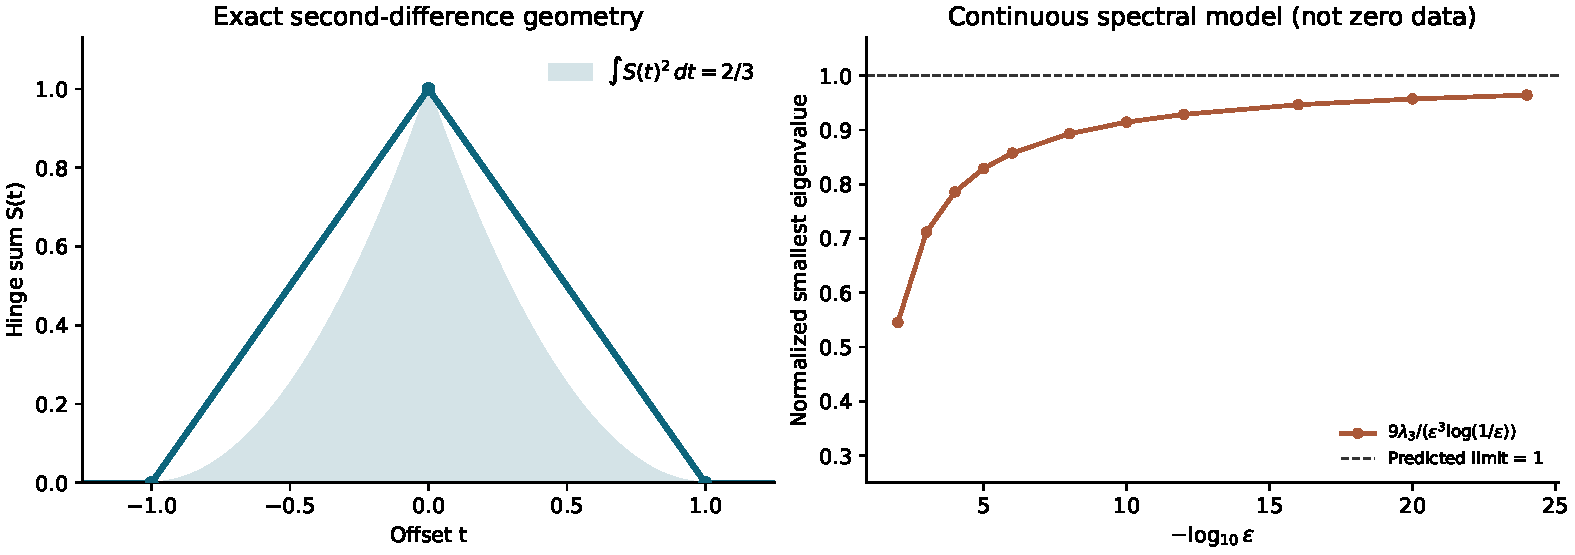
\includegraphics[width=\linewidth]{figures/coalescence_geometry.pdf}
\caption{Left: the second-difference hinge function for offsets
$(-1,0,1)$; the shaded area is its squared integral $2/3$.
Right: a continuous spectral model with the correct leading zero
density, explicitly distinguished from actual zero data. It illustrates
the predicted cubic logarithmic normalization.}
\label{fig:model}
\end{figure}

\paragraph{Formal status and novelty.}
No Lean build of the new theorem was performed, and no generated
\texttt{.lean} file is presented as certified. The natural formalization
sequence is: the scalar explicit formula and means; Montgomery's
uniform pair estimate; the frozen-kernel local comparison; scaled
Stieltjes measures; the finite spline identity; and the block-matrix
argument. The upstream RH theorem is a separate dependency. The
standard spline identities, Parseval, min--max, Schur complements and
classical analytic inputs receive no novelty claim. The proposed
contribution is the explicit arithmetic coalescence theorem and the
prediction and difference consequences, with unknown multiplicities
retained throughout.

\paragraph{Scope of sharpness.}
The exponents and logarithm are forced by positive lower and finite
upper bounds. The factor $4/3$ comes from the elementary squared-sinc
test. Optimized positive pair-correlation kernels can improve that
numerical factor; pursuing the optimal factor is outside this note.
No effective numerical onset for the asymptotic inequalities is
claimed. All observation nodes, the number of observations, the
difference order and any deleted frequency set are fixed before
$\eps\to0$.

\begin{thebibliography}{99}
\bibitem{grh}
L. Sernau and collaborators,
\emph{GRH for Dirichlet $L$-functions, in Lean 4},
commit \texttt{72fead102f663d5c7a407964a13dc0cf9d977207},
25 November 2026.
\url{https://github.com/lsernau/grh-lean}.
Inspected: \path{grh/GUIDE.md}, \path{grh/src/Statements.lean},
\path{grh/src/Main.lean}, and the main inequality, one-sided bound,
prime-error and zero-criterion source files. Exact pinned paths are in
the provenance manifest.

\bibitem{sutherland}
A. Sutherland,
\emph{Verification files for the shorter Lean proof of RH and GRH},
report updated 26 November 2026, 01:52 UTC.
\url{https://math.mit.edu/~drew/shortgrh/}.

\bibitem{catalogue}
V. Reshetnikov, \emph{ProveIt: Generalized Riemann Hypothesis research
catalogue}, inspected at commit
\texttt{2ccd1e24d0f3fa8a5268c864f66a6b1b4e2d0d59}.
\url{https://github.com/VladimirReshetnikov/ProveIt/tree/main/Analysis/GeneralizedRiemannHypothesis}.

\bibitem{prior}
ProveIt research packet,
\emph{Strict multiscale covariance of smoothed prime errors},
26 November 2026, \path{report.tex} in
\path{Analysis/GeneralizedRiemannHypothesis/docs/incoming/grh_multiscale_covariance.zip},
at the ProveIt commit in \cite{catalogue}. The final research questions
ask for the sharp merging-scale decay. The complete immutable archive
URL is recorded in \path{provenance/source_manifest.json}.

\bibitem{wiki}
Wikipedia contributors, \emph{Riemann hypothesis}, accessed
26 November 2026.
\url{https://en.wikipedia.org/wiki/Riemann_hypothesis}.
Used as the requested overview; proof inputs are given in the primary
references below.

\bibitem{montgomery}
H. L. Montgomery, The pair correlation of zeros of the zeta function,
\emph{Analytic Number Theory}, Proceedings of Symposia in Pure
Mathematics \textbf{24}, American Mathematical Society, 1973,
181--193. In particular the theorem on p.~181, equation~(6) on p.~182,
and the proof on pp.~191--192.
\url{https://public.websites.umich.edu/hlm/paircor1.pdf}.

\bibitem{CGG}
J. B. Conrey, A. Ghosh and S. M. Gonek,
Simple zeros of the Riemann zeta-function,
\emph{Proceedings of the London Mathematical Society} (3)
\textbf{76} (1998), 497--522. The introduction explicitly states the
classical squared-multiplicity estimate and its counting convention.
\url{https://sas.rochester.edu/mth/people/faculty/gonek-steve/assets/pdf/simplezeros.pdf}.

\bibitem{BU}
S. Barthelm\'e and K. Usevich,
Spectral properties of kernel matrices in the flat limit,
\emph{SIAM Journal on Matrix Analysis and Applications}
\textbf{42} (2021), 17--57.
\url{https://doi.org/10.1137/19M129677X}.
Preprint consulted: arXiv:1910.14067v3, 27 March 2025,
especially Theorems~4.5--4.6.
\url{https://arxiv.org/abs/1910.14067}.

\bibitem{kouk}
D. Koukoulopoulos, \emph{The Distribution of Prime Numbers},
Graduate Studies in Mathematics \textbf{203}, American Mathematical
Society, 2019, Chapters~5--8 and~11, and Appendices~A--B.
\url{https://dms.umontreal.ca/~koukoulo/documents/publications/primes.pdf}.
\end{thebibliography}
\end{document}
